

\section{Results}



\subsection{Part 1: Magnetic field strength and current}

\begin{figure}
    \centering
    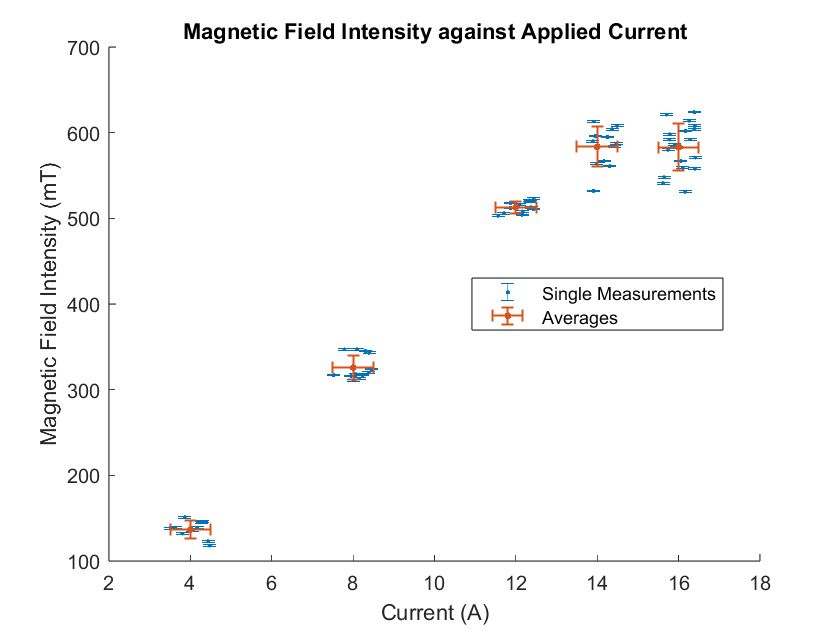
\includegraphics[width=0.8\textwidth]{Results/Figures/Magnetic_Field_vs_Current_jitter.png}
    \caption{Magnetic Field Strength vs Current Jitter Plot}
    \label{fig:magnetic_field_vs_current_jitter}
\end{figure}
\begin{figure}
    \centering
    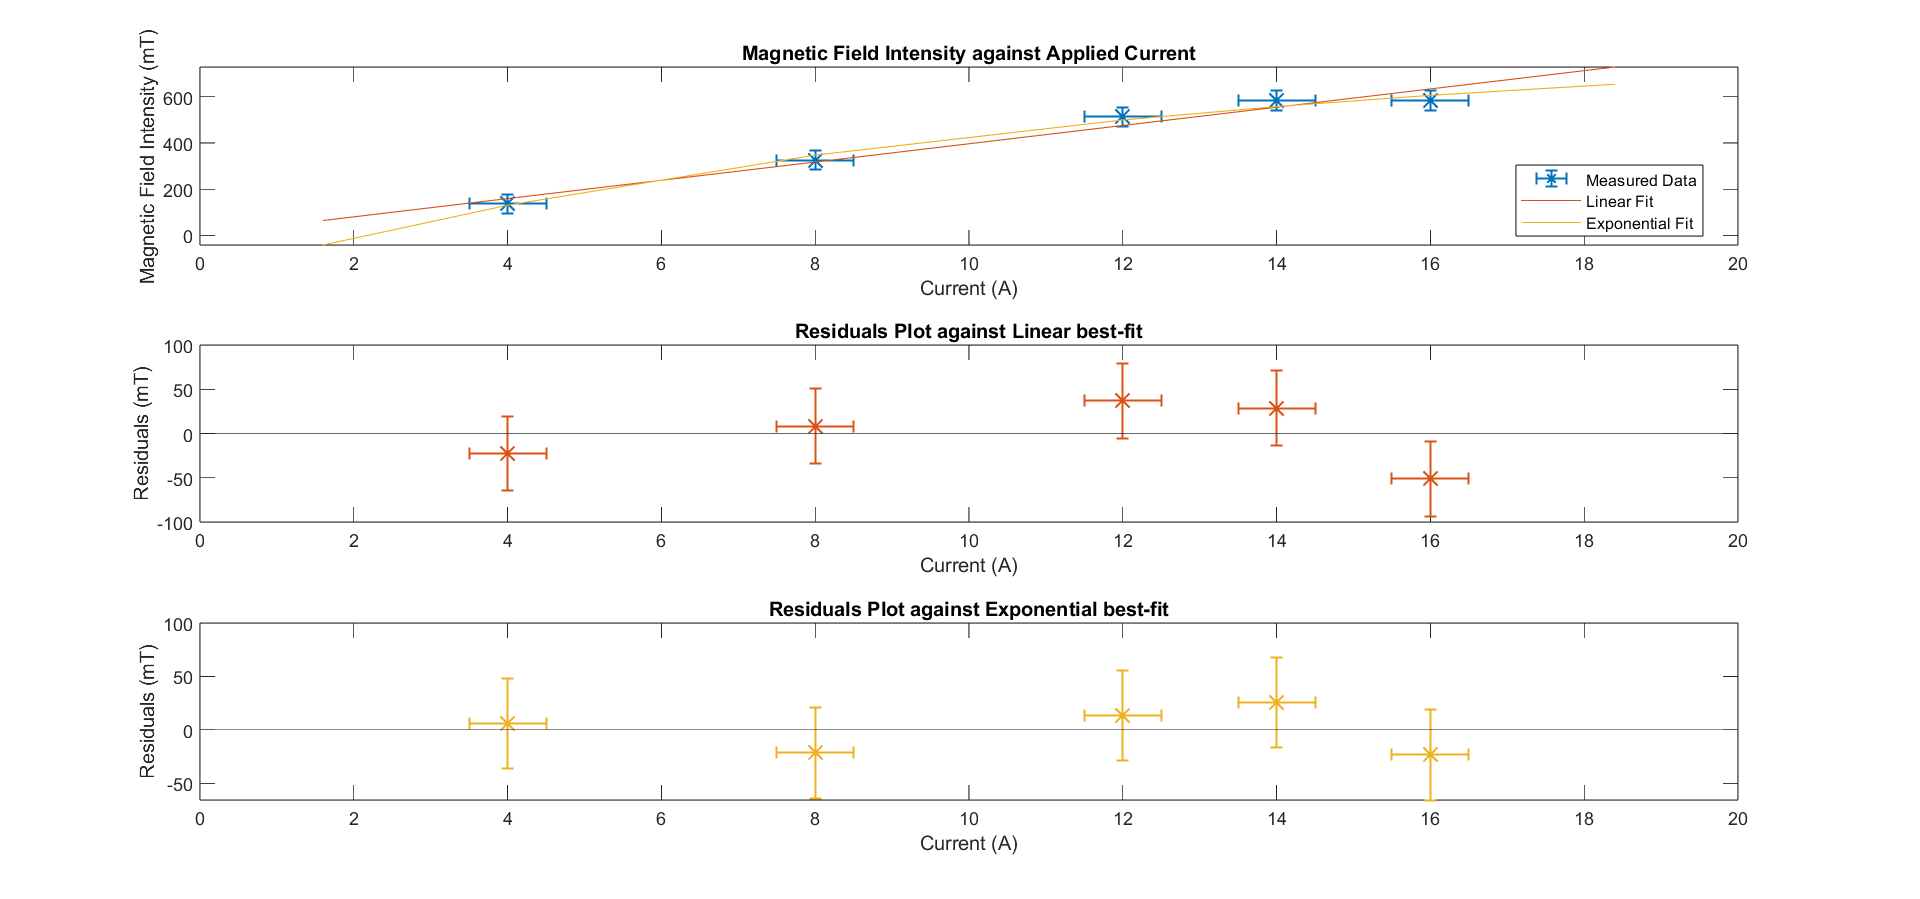
\includegraphics[width=0.8\textwidth]{Results/Figures/Magnetic_Field_vs_Current.png}
    \caption{Magnetic Field Strength vs Current Regression Plots for Linear and Exponential fits}
    \label{fig:magnetic_field_vs_current}
\end{figure}
Figure \ref{fig:magnetic_field_vs_current_jitter} shows the magnetic field strength as a function of the current supplied to the electromagnet, showing the averages and standard deviations at each measured current value. Then, using these averages, figure \ref{fig:magnetic_field_vs_current} applies a linear and exponential fit to the data. These fits are given by:
\begin{gather*}
    B = (1 \pm 51) + (39.6 \pm 4.4)I~[mT] \quad \chi^2 / \nu = 40.0 / 3 = 13.3 \\
    B = (-1040 \pm 150) exp (-0.089 \pm 0.051 * I) + (860 \pm 260)~[mT] \\
    \chi^2 / \nu = 17.7 / 2 = 8.85
\end{gather*}
The linear fit has a reduced chi-squared value of 13.3, which is quite high and the residuals show a clear downwards-curving pattern, showing that a linear fit is not. The exponential fit has a lower reduced chi-squared value of 8.85 and the residuals show a more random pattern, indicating that the exponential fit is a better fit to the data.



After adjusting the magnet poles, several measurements of the magnetic filed intensity were taken using the Gauss meter. The results are shown in the table below.

\subsection{Part 2: Observing the Zeeman split perpendicularly to the magnetic field}

These measurements result in an average value of: $B = 136.70 \pm 10$ mT.

The field current and pole positions were not changed throughout the experiment, so we assume the
magnetic field intensity to be constant for this specific trial.

\begin{table}
    \begin{adjustwidth}{-130pt}{-130pt}
        \centering
        \begin{tabular}{|l|l|l|l|l|l|}
            \hline
            {\ul \textbf{Trial:}}        & {\ul Trial 1} & {\ul Trial 2}  & {\ul Trial 3}  & {\ul Trial 4}  & {\ul Trial 5} \\ \hline
            {\ul \textbf{Field Value:} } & $151 \pm 0.5$ & $146  \pm 0.5$ & $145  \pm 0.5$ & $139  \pm 0.5$ & $139 \pm 0.5$ \\ \hline
        \end{tabular} \\
        \begin{tabular}{|l|l|l|l|l|l|}
            \hline
            {\ul \textbf{Trial:}}        & {\ul Trial 6} & {\ul Trial 7} & {\ul Trial 8} & {\ul Trial 9} & {\ul Average}  \\ \hline
            {\ul \textbf{Field Value:} } & $138 \pm 0.5$ & $136 \pm 0.5$ & $132 \pm 0.5$ & $123 \pm 0.5$ & $136.7 \pm 10$ \\ \hline
        \end{tabular}

        \caption{Magnetic field intensity measurments in mT for trial 1: 4A current}


    \end{adjustwidth}

\end{table}


\def\lineUncertainty{0.05}

% Source: Raw_Data_Part_1.tgn
\begin{table}
    \begin{adjustwidth}{-100pt}{-100pt}
        \centering
        \begin{tabular}{|l|l|l|l|l|l|}
            \hline
            {\ul Trial}   & Line Position                & Upper edge position          & Lower edge position          & $\Delta$ width              & Zeeman Shift                 \\ \hline
            {\ul 1}       & $0.23 \pm \lineUncertainty$  & $0.02 \pm \lineUncertainty$  & $-0.08 \pm \lineUncertainty$ & $0.10 \pm \lineUncertainty$ & $0.05 \pm \lineUncertainty$  \\ \hline
            {\ul 2}       & $0.0 \pm \lineUncertainty$   & $-0.22 \pm \lineUncertainty$ & $-0.31 \pm \lineUncertainty$ & $0.09 \pm \lineUncertainty$ & $0.045 \pm \lineUncertainty$ \\ \hline
            {\ul 3}       & $-0.24 \pm \lineUncertainty$ & $-0.41 \pm \lineUncertainty$ & $-0.49 \pm \lineUncertainty$ & $0.08 \pm \lineUncertainty$ & $0.04 \pm \lineUncertainty$  \\ \hline
            {\ul 4}       & $-0.41 \pm \lineUncertainty$ & $-0.59 \pm \lineUncertainty$ & $-0.68 \pm \lineUncertainty$ & $0.09 \pm \lineUncertainty$ & $0.045 \pm \lineUncertainty$ \\ \hline
            {\ul 5}       & $-0.6 \pm \lineUncertainty$  & $-0.73 \pm \lineUncertainty$ & $-0.82 \pm \lineUncertainty$ & $0.09 \pm \lineUncertainty$ & $0.045 \pm \lineUncertainty$ \\ \hline
            {\ul 6}       & $-0.76 \pm \lineUncertainty$ & $-0.90 \pm \lineUncertainty$ & $-0.96 \pm \lineUncertainty$ & $0.06 \pm \lineUncertainty$ & $0.03 \pm \lineUncertainty$  \\ \hline
            {\ul Average} &                              &                              &                              &                             & $0.043 \pm 0.01$             \\ \hline
        \end{tabular}
    \end{adjustwidth}
    \caption{Zeeman shift measurments for trial 1: 4A current}
\end{table}

Next, the measurments are repeated for different current values. The results are shown in the tables below.

\begin{table}
    \begin{adjustwidth}{-130pt}{-130pt}
        \centering
        \begin{tabular}{|l|l|l|l|l|l|}
            \hline
            {\ul \textbf{Trial:}}        & {\ul Trial 1} & {\ul Trial 2}  & {\ul Trial 3}  & {\ul Trial 4}  & {\ul Trial 5} \\ \hline
            {\ul \textbf{Field Value:} } & $347 \pm 0.5$ & $345  \pm 0.5$ & $343  \pm 0.5$ & $347  \pm 0.5$ & $320 \pm 0.5$ \\ \hline
        \end{tabular} \\
        \vspace{0.2cm} % Add some space between the tables
        \begin{tabular}{|l|l|l|l|l|l|}
            \hline
            {\ul \textbf{Trial:}}        & {\ul Trial 6} & {\ul Trial 7} & {\ul Trial 8} & {\ul Trial 9} & {\ul Trial 10} \\ \hline
            {\ul \textbf{Field Value:} } & $324 \pm 0.5$ & $318 \pm 0.5$ & $317 \pm 0.5$ & $318 \pm 0.5$ & $317 \pm 0.5$  \\ \hline
        \end{tabular} \\
        \vspace{0.2cm} % Add some space between the tables
        \begin{tabular}{|l|l|l|l|l|}
            \hline
            {\ul \textbf{Trial:}}        & {\ul Trial 11} & {\ul Trial 12} & {\ul Trial 13} & {\ul Average}   \\ \hline
            {\ul \textbf{Field Value:} } & $316 \pm 0.5$  & $313 \pm 0.5$  & $311 \pm 0.5$  & $325.85 \pm 14$ \\ \hline
        \end{tabular}

        \caption{Magnetic field intensity measurments in mT for trial 2: 6A current}

    \end{adjustwidth}
\end{table}


\begin{table}
    \begin{adjustwidth}{-100pt}{-100pt}
        \centering
        \begin{tabular}{|l|l|l|l|l|l|}
            \hline
            {\ul Trial}   & Line Position                & Upper edge position          & Lower edge position          & $\Delta$ width              & Zeeman Shift                 \\ \hline
            {\ul 1}       & $0.23 \pm \lineUncertainty$  & $0.03 \pm \lineUncertainty$  & $-0.09 \pm \lineUncertainty$ & $0.12 \pm \lineUncertainty$ & $0.06 \pm \lineUncertainty$  \\ \hline
            {\ul 2}       & $0.0 \pm \lineUncertainty$   & $-0.21 \pm \lineUncertainty$ & $-0.33 \pm \lineUncertainty$ & $0.12 \pm \lineUncertainty$ & $0.06 \pm \lineUncertainty$  \\ \hline
            {\ul 3}       & $-0.24 \pm \lineUncertainty$ & $-0.41 \pm \lineUncertainty$ & $-0.50 \pm \lineUncertainty$ & $0.09 \pm \lineUncertainty$ & $0.045 \pm \lineUncertainty$ \\ \hline
            {\ul 4}       & $-0.41 \pm \lineUncertainty$ & $-0.57 \pm \lineUncertainty$ & $-0.66 \pm \lineUncertainty$ & $0.09 \pm \lineUncertainty$ & $0.045 \pm \lineUncertainty$ \\ \hline
            {\ul 5}       & $-0.6 \pm \lineUncertainty$  & $-0.73 \pm \lineUncertainty$ & $-0.83 \pm \lineUncertainty$ & $0.10 \pm \lineUncertainty$ & $0.05 \pm \lineUncertainty$  \\ \hline
            {\ul 6}       & $-0.76 \pm \lineUncertainty$ & $-0.87 \pm \lineUncertainty$ & $-0.96 \pm \lineUncertainty$ & $0.09 \pm \lineUncertainty$ & $0.045 \pm \lineUncertainty$ \\ \hline
            {\ul Average} &                              &                              &                              &                             & $0.051 \pm 0.01$             \\ \hline
        \end{tabular}
    \end{adjustwidth}

    \caption{Zeeman shift measurments for trial 2: 6A current}


\end{table}


\begin{table}
    \begin{adjustwidth}{-130pt}{-130pt}
        \centering
        \begin{tabular}{|l|l|l|l|l|l|}
            \hline
            {\ul \textbf{Trial:}}        & {\ul Trial 1} & {\ul Trial 2}  & {\ul Trial 3}  & {\ul Trial 4}  & {\ul Trial 5} \\ \hline
            {\ul \textbf{Field Value:} } & $512 \pm 0.5$ & $523  \pm 0.5$ & $521  \pm 0.5$ & $520  \pm 0.5$ & $518 \pm 0.5$ \\ \hline
        \end{tabular} \\
        \vspace{0.2cm} % Add some space between the tables
        \begin{tabular}{|l|l|l|l|l|l|}
            \hline
            {\ul \textbf{Trial:}}        & {\ul Trial 6} & {\ul Trial 7} & {\ul Trial 8} & {\ul Trial 9} & {\ul Trial 10} \\ \hline
            {\ul \textbf{Field Value:} } & $516 \pm 0.5$ & $513 \pm 0.5$ & $511 \pm 0.5$ & $508 \pm 0.5$ & $506 \pm 0.5$  \\ \hline
        \end{tabular} \\
        \vspace{0.2cm} % Add some space between the tables
        \begin{tabular}{|l|l|l|l|}
            \hline
            {\ul \textbf{Trial:}}        & {\ul Trial 11} & {\ul Trial 12} & {\ul Average}    \\ \hline
            {\ul \textbf{Field Value:} } & $504 \pm 0.5$  & $503 \pm 0.5$  & $512.92 \pm 6.5$ \\ \hline
        \end{tabular}

        \caption{Magnetic field intensity measurments in mT for trial 3: 12A current}

    \end{adjustwidth}
\end{table}

\begin{table}
    \begin{adjustwidth}{-100pt}{-100pt}
        \centering
        \begin{tabular}{|l|l|l|l|l|l|}
            \hline
            {\ul Trial}   & Line Position                & Upper edge position          & Lower edge position          & $\Delta$ width              & Zeeman Shift                 \\ \hline
            {\ul 1}       & $0.23 \pm \lineUncertainty$  & $0.06 \pm \lineUncertainty$  & $-0.13 \pm \lineUncertainty$ & $0.19 \pm \lineUncertainty$ & $0.095 \pm \lineUncertainty$ \\ \hline
            {\ul 2}       & $0.0 \pm \lineUncertainty$   & $-0.19 \pm \lineUncertainty$ & $-0.33 \pm \lineUncertainty$ & $0.14 \pm \lineUncertainty$ & $0.07 \pm \lineUncertainty$  \\ \hline
            {\ul 3}       & $-0.24 \pm \lineUncertainty$ & $-0.38 \pm \lineUncertainty$ & $-0.51 \pm \lineUncertainty$ & $0.13 \pm \lineUncertainty$ & $0.065 \pm \lineUncertainty$ \\ \hline
            {\ul 4}       & $-0.41 \pm \lineUncertainty$ & $-0.56 \pm \lineUncertainty$ & $-0.70 \pm \lineUncertainty$ & $0.14 \pm \lineUncertainty$ & $0.07 \pm \lineUncertainty$  \\ \hline
            {\ul 5}       & $-0.6 \pm \lineUncertainty$  & $-0.73 \pm \lineUncertainty$ & $-0.85 \pm \lineUncertainty$ & $0.12 \pm \lineUncertainty$ & $0.06 \pm \lineUncertainty$  \\ \hline
            {\ul 6}       & $-0.76 \pm \lineUncertainty$ & $-0.88 \pm \lineUncertainty$ & $-0.97 \pm \lineUncertainty$ & $0.09 \pm \lineUncertainty$ & $0.045 \pm \lineUncertainty$ \\ \hline
            {\ul Average} &                              &                              &                              &                             & $0.067 \pm 0.01$             \\ \hline
        \end{tabular}
    \end{adjustwidth}

    \caption{Zeeman shift measurments for trial 3: 12A current}

\end{table}


\begin{table}
    \begin{adjustwidth}{-130pt}{-130pt}
        \centering
        \begin{tabular}{|l|l|l|l|l|l|}
            \hline
            {\ul \textbf{Trial:}}        & {\ul Trial 1} & {\ul Trial 2}  & {\ul Trial 3}  & {\ul Trial 4}  & {\ul Trial 5} \\ \hline
            {\ul \textbf{Field Value:} } & $532 \pm 0.5$ & $567  \pm 0.5$ & $584  \pm 0.5$ & $561  \pm 0.5$ & $564 \pm 0.5$ \\ \hline
        \end{tabular} \\
        \vspace{0.2cm} % Add some space between the tables
        \begin{tabular}{|l|l|l|l|l|l|}
            \hline
            {\ul \textbf{Trial:}}        & {\ul Trial 6} & {\ul Trial 7} & {\ul Trial 8} & {\ul Trial 9} & {\ul Trial 10} \\ \hline
            {\ul \textbf{Field Value:} } & $595 \pm 0.5$ & $613 \pm 0.5$ & $587 \pm 0.5$ & $608 \pm 0.5$ & $604 \pm 0.5$  \\ \hline
        \end{tabular} \\
        \vspace{0.2cm} % Add some space between the tables
        \begin{tabular}{|l|l|l|l|}
            \hline
            {\ul \textbf{Trial:}}        & {\ul Trial 11} & {\ul Trial 12} & {\ul Average}   \\ \hline
            {\ul \textbf{Field Value:} } & $590 \pm 0.5$  & $596 \pm 0.5$  & $583.42 \pm 22$ \\ \hline
        \end{tabular}

        \caption{Magnetic field intensity measurments in mT for trial 4: 14A current}

    \end{adjustwidth}
\end{table}

\begin{table}
    \begin{adjustwidth}{-100pt}{-100pt}
        \centering
        \begin{tabular}{|l|l|l|l|l|l|}
            \hline
            {\ul Trial}   & Line Position                & Upper edge position          & Lower edge position          & $\Delta$ width              & Zeeman Shift                 \\ \hline
            {\ul 1}       & $0.23 \pm \lineUncertainty$  & $0.08 \pm \lineUncertainty$  & $-0.11 \pm \lineUncertainty$ & $0.19 \pm \lineUncertainty$ & $0.095 \pm \lineUncertainty$ \\ \hline
            {\ul 2}       & $0.0 \pm \lineUncertainty$   & $-0.19 \pm \lineUncertainty$ & $-0.37 \pm \lineUncertainty$ & $0.18 \pm \lineUncertainty$ & $0.09 \pm \lineUncertainty$  \\ \hline
            {\ul 3}       & $-0.24 \pm \lineUncertainty$ & $-0.40 \pm \lineUncertainty$ & $-0.54 \pm \lineUncertainty$ & $0.14 \pm \lineUncertainty$ & $0.07 \pm \lineUncertainty$  \\ \hline
            {\ul 4}       & $-0.41 \pm \lineUncertainty$ & $-0.59 \pm \lineUncertainty$ & $-0.67 \pm \lineUncertainty$ & $0.08 \pm \lineUncertainty$ & $0.04 \pm \lineUncertainty$  \\ \hline
            {\ul 5}       & $-0.6 \pm \lineUncertainty$  & $-0.72 \pm \lineUncertainty$ & $-0.83 \pm \lineUncertainty$ & $0.11 \pm \lineUncertainty$ & $0.055 \pm \lineUncertainty$ \\ \hline
            {\ul 6}       & $-0.76 \pm \lineUncertainty$ & $-0.86 \pm \lineUncertainty$ & $-0.96 \pm \lineUncertainty$ & $0.10 \pm \lineUncertainty$ & $0.05 \pm \lineUncertainty$  \\ \hline
            {\ul Average} &                              &                              &                              &                             & $0.067 \pm 0.02$             \\ \hline
        \end{tabular}
    \end{adjustwidth}

    \caption{Zeeman shift measurments for trial 4: 14A current}

\end{table}



\begin{table}
    \begin{adjustwidth}{-130pt}{-130pt}
        \centering
        \begin{tabular}{|l|l|l|l|l|l|}
            \hline
            {\ul \textbf{Trial:}}        & {\ul Trial 1} & {\ul Trial 2}  & {\ul Trial 3}  & {\ul Trial 4}  & {\ul Trial 5} \\ \hline
            {\ul \textbf{Field Value:} } & $580 \pm 0.5$ & $592  \pm 0.5$ & $624  \pm 0.5$ & $571  \pm 0.5$ & $567 \pm 0.5$ \\ \hline
        \end{tabular} \\
        \vspace{0.2cm} % Add some space between the tables
        \begin{tabular}{|l|l|l|l|l|l|}
            \hline
            {\ul \textbf{Trial:}}        & {\ul Trial 6} & {\ul Trial 7} & {\ul Trial 8} & {\ul Trial 9} & {\ul Trial 10} \\ \hline
            {\ul \textbf{Field Value:} } & $559 \pm 0.5$ & $548 \pm 0.5$ & $558 \pm 0.5$ & $583 \pm 0.5$ & $621 \pm 0.5$  \\ \hline
        \end{tabular} \\
        \vspace{0.2cm} % Add some space between the tables
        \begin{tabular}{|l|l|l|l|l|l|}
            \hline
            {\ul \textbf{Trial:}}        & {\ul Trial 11} & {\ul Trial 12} & {\ul Trial 13} & {\ul Trial 14} & {\ul Trial 15} \\ \hline
            {\ul \textbf{Field Value:} } & $608 \pm 0.5$  & $614 \pm 0.5$  & $604 \pm 0.5$  & $598 \pm 0.5$  & $602 \pm 0.5$  \\ \hline
        \end{tabular} \\
        \vspace{0.2cm} % Add some space between the tables
        \begin{tabular}{|l|l|l|l|}
            \hline
            {\ul \textbf{Trial:}}        & {\ul Trial 16} & {\ul Trial 17} & {\ul Average}      \\ \hline
            {\ul \textbf{Field Value:} } & $531 \pm 0.5$  & $541 \pm 0.5$  & $583.11 \pm 26.37$ \\ \hline
        \end{tabular}

        \caption{Magnetic field intensity measurments in mT for trial 5: 16A current}

    \end{adjustwidth}
\end{table}


\begin{table}
    \begin{adjustwidth}{-100pt}{-100pt}
        \centering
        \begin{tabular}{|l|l|l|l|l|l|}
            \hline
            {\ul Trial}   & Line Position                & Upper edge position          & Lower edge position          & $\Delta$ width              & Zeeman Shift                 \\ \hline
            {\ul 1}       & $0.23 \pm \lineUncertainty$  & $0.09 \pm \lineUncertainty$  & $-0.14 \pm \lineUncertainty$ & $0.23 \pm \lineUncertainty$ & $0.115 \pm \lineUncertainty$ \\ \hline
            {\ul 2}       & $0.0 \pm \lineUncertainty$   & $-0.19 \pm \lineUncertainty$ & $-0.35 \pm \lineUncertainty$ & $0.16 \pm \lineUncertainty$ & $0.08 \pm \lineUncertainty$  \\ \hline
            {\ul 3}       & $-0.24 \pm \lineUncertainty$ & $-0.40 \pm \lineUncertainty$ & $-0.51 \pm \lineUncertainty$ & $0.11 \pm \lineUncertainty$ & $0.055 \pm \lineUncertainty$ \\ \hline
            {\ul 4}       & $-0.41 \pm \lineUncertainty$ & $-0.56 \pm \lineUncertainty$ & $-0.68 \pm \lineUncertainty$ & $0.12 \pm \lineUncertainty$ & $0.06 \pm \lineUncertainty$  \\ \hline
            {\ul 5}       & $-0.6 \pm \lineUncertainty$  & $-0.74 \pm \lineUncertainty$ & $-0.83 \pm \lineUncertainty$ & $0.09 \pm \lineUncertainty$ & $0.045 \pm \lineUncertainty$ \\ \hline
            {\ul 6}       & $-0.76 \pm \lineUncertainty$ & $-0.87 \pm \lineUncertainty$ & $-0.97 \pm \lineUncertainty$ & $0.10 \pm \lineUncertainty$ & $0.05 \pm \lineUncertainty$  \\ \hline
            {\ul Average} &                              &                              &                              &                             & $0.067 \pm 0.02$             \\ \hline
        \end{tabular}
    \end{adjustwidth}

    \caption{Zeeman shift measurments for trial 5: 16A current}

\end{table}

\subsection{Part 3: Observing the linearity of the Zeeman shift with respect to the field strength}

Now, we plot the previouslt obtained values in a scatter plot and compare it to a linear fit.

\begin{figure}
    \centering
    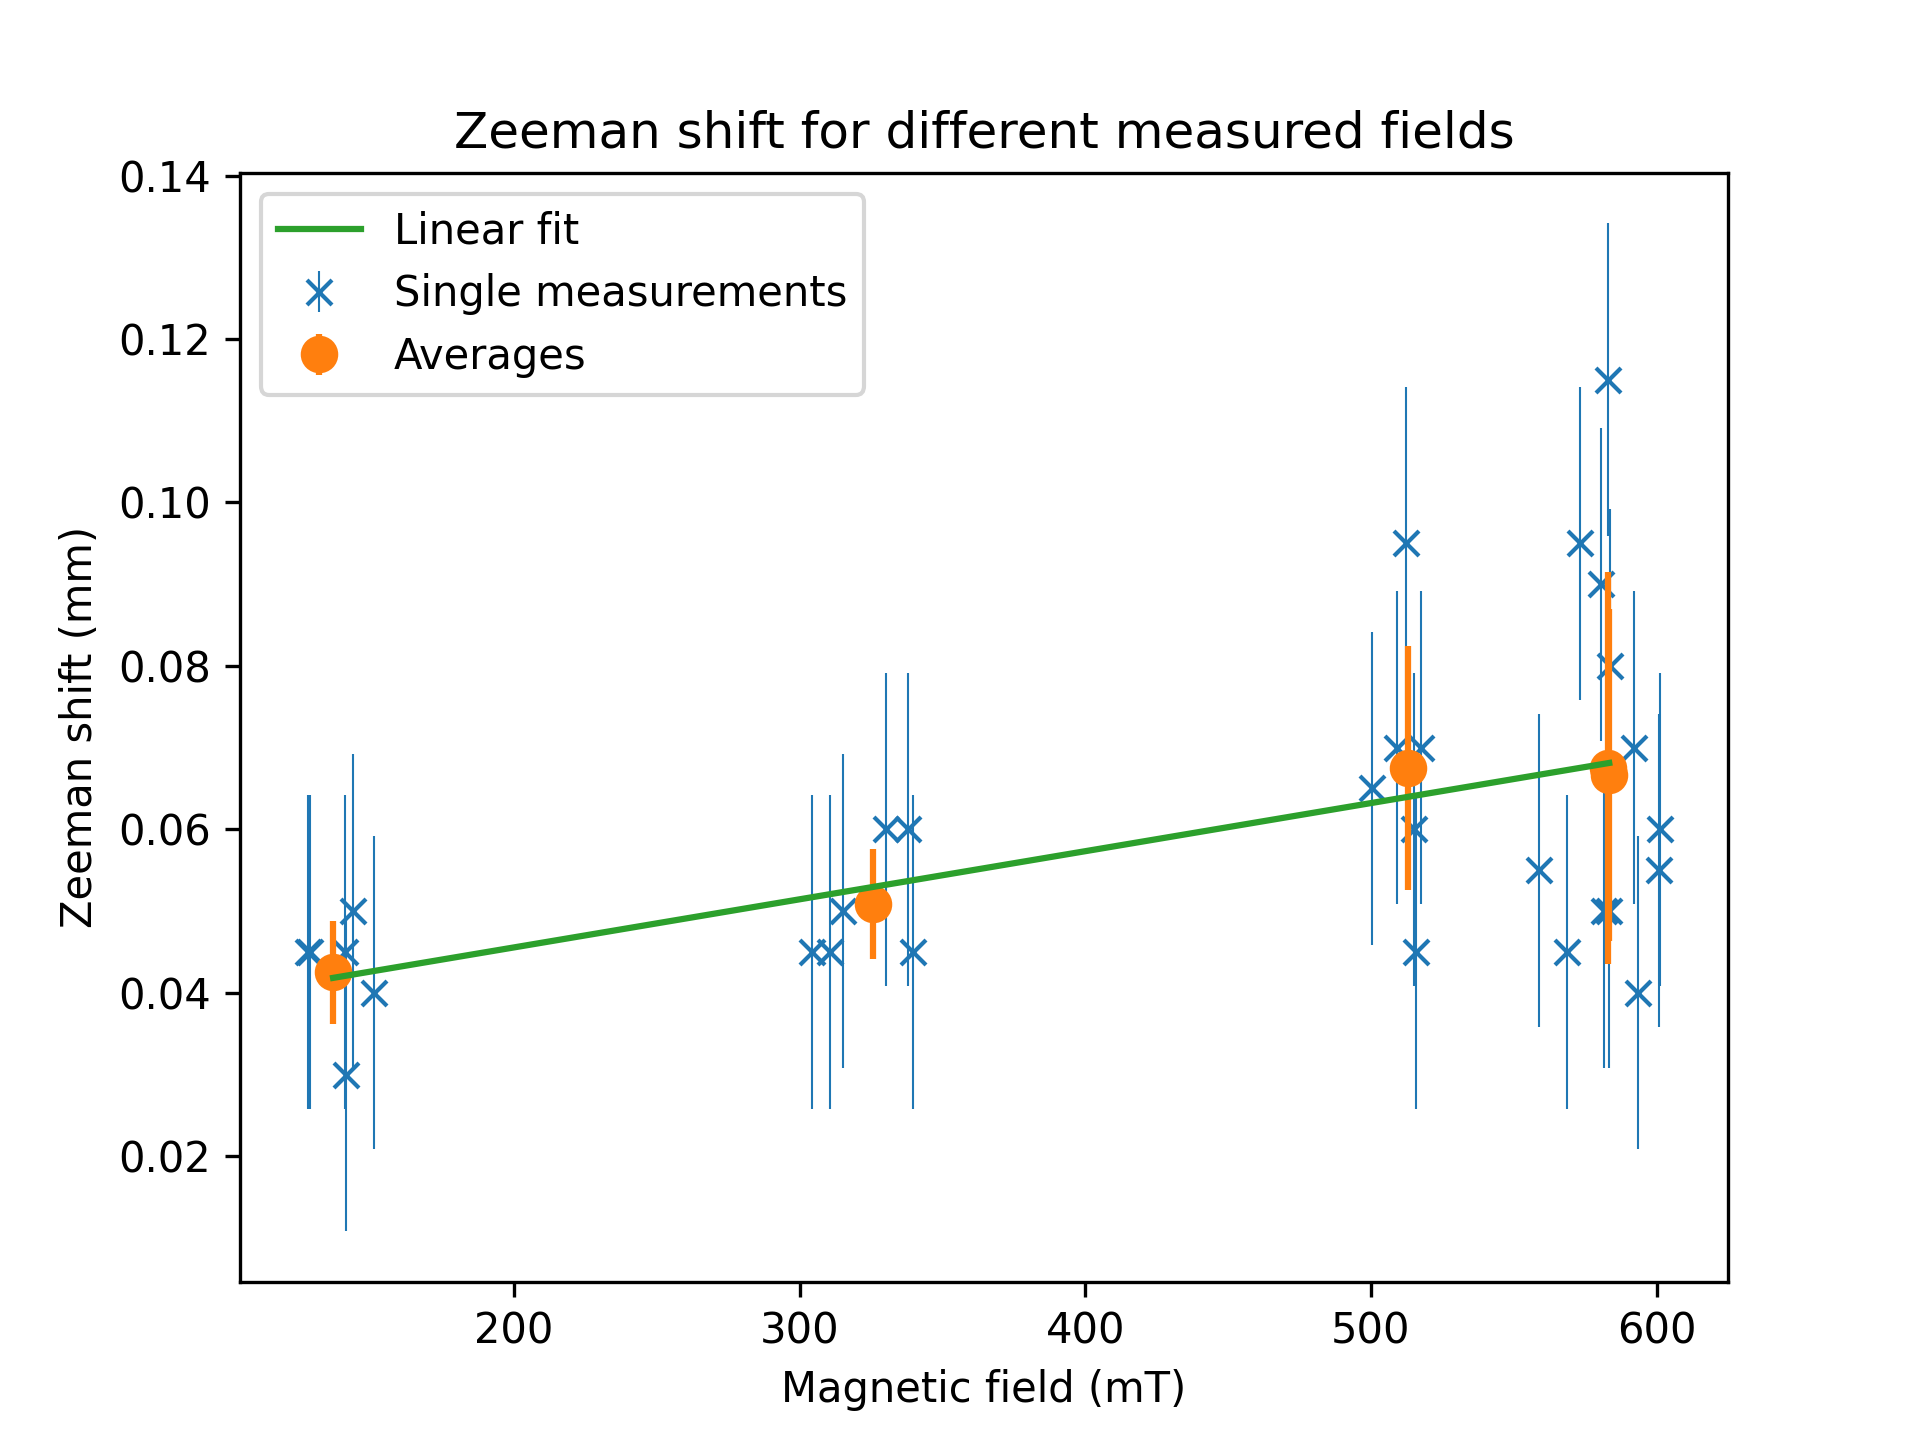
\includegraphics[width=0.8\textwidth]{Results/img/zeeman_shift_scatter.png}
    \caption{Zeeman Shift vs Magnetic Field Intensity}
\end{figure}

\begin{figure}
    \centering
    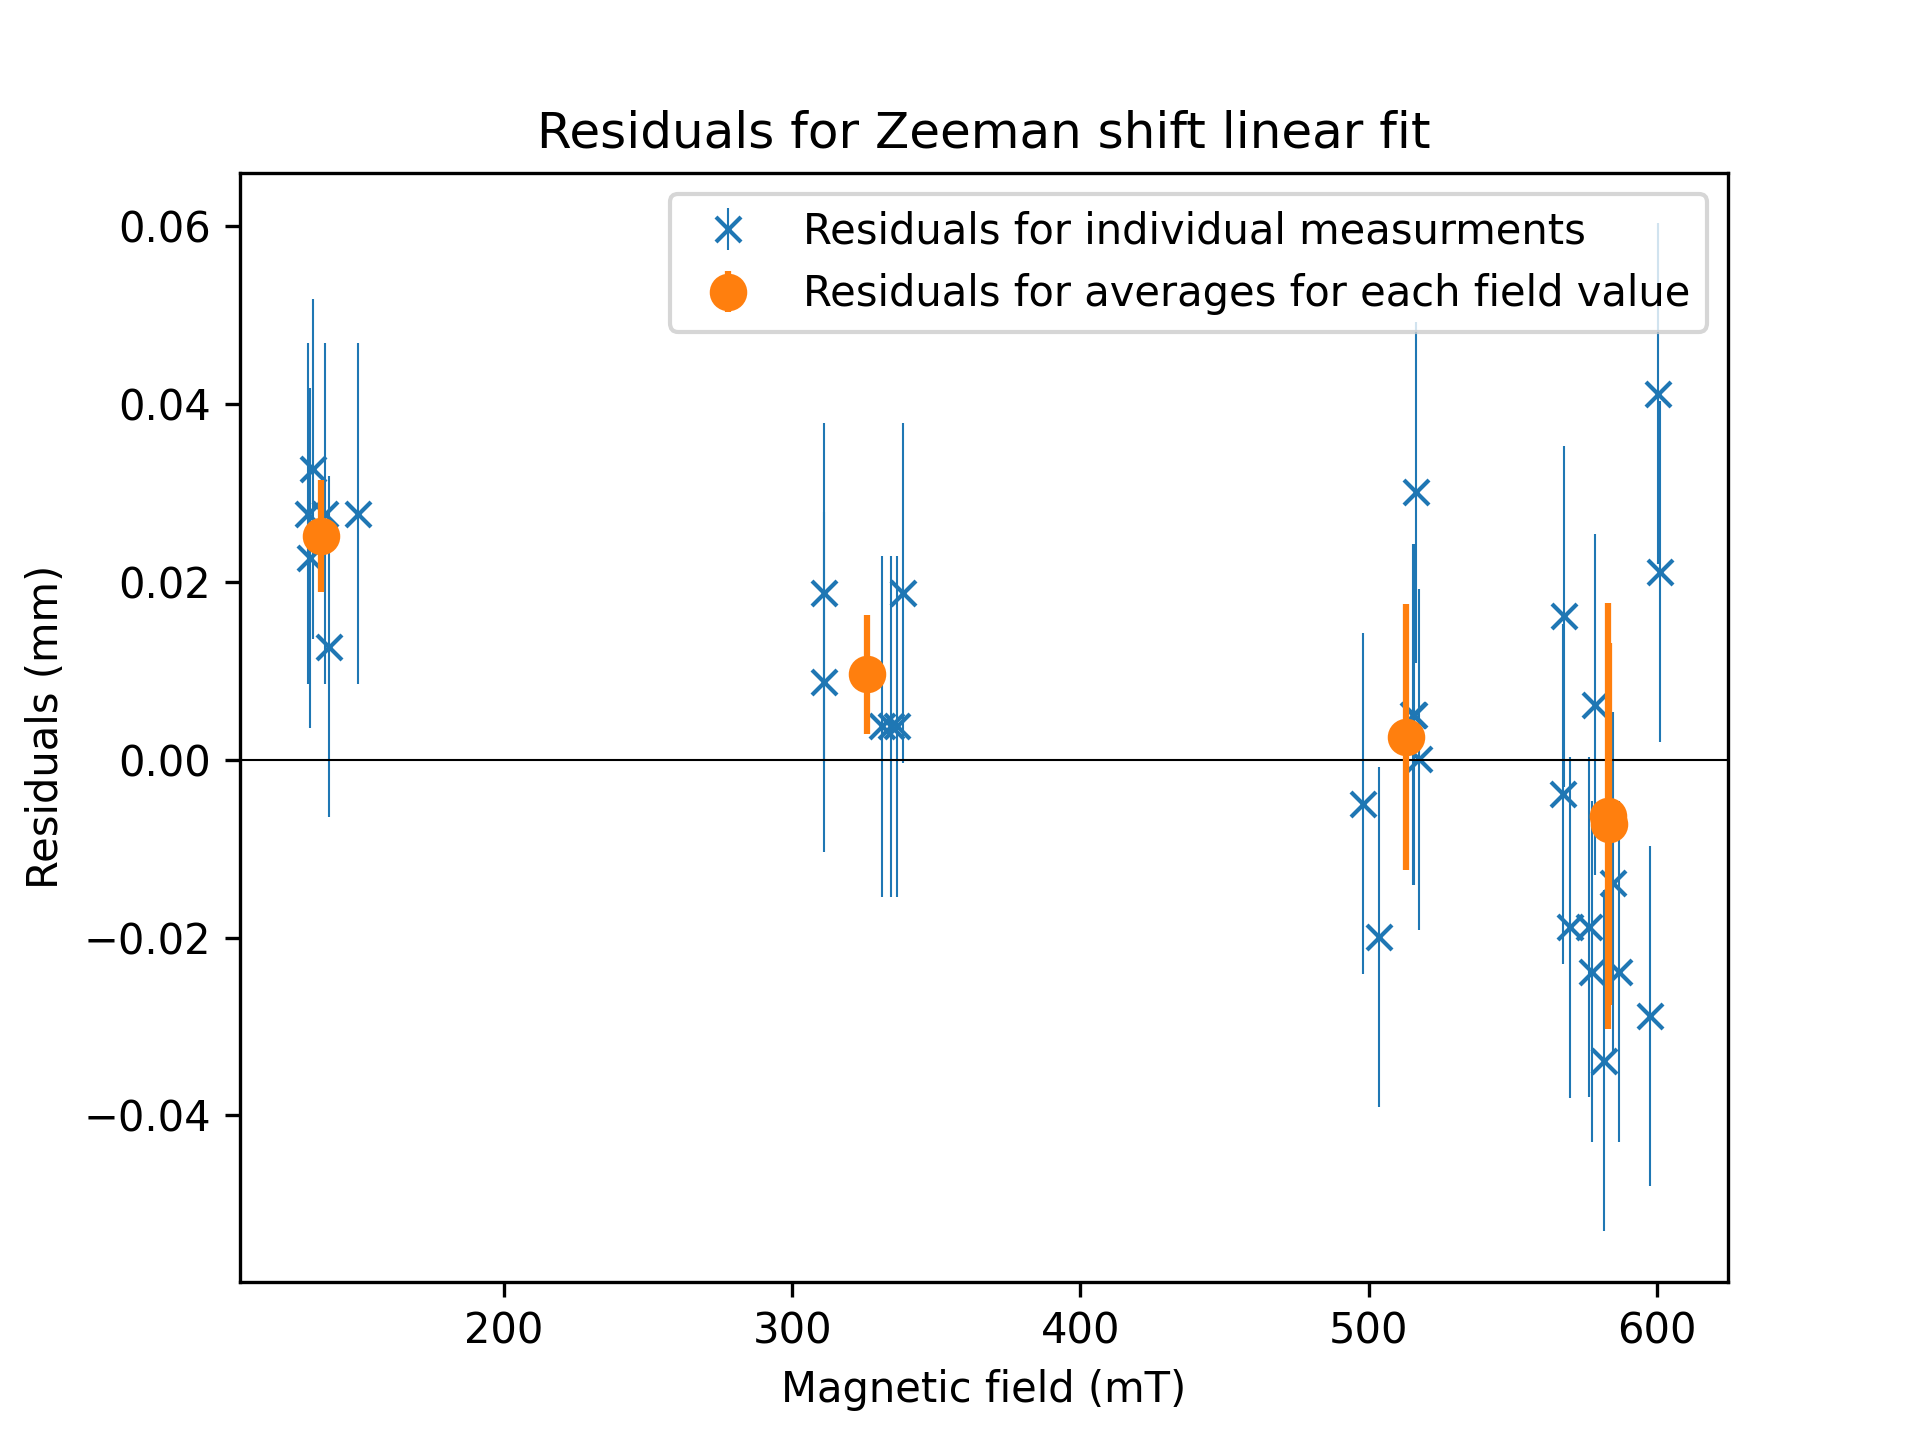
\includegraphics[width=0.8\textwidth]{Results/img/zeeman_shift_residuals.png}
    \caption{Zeeman Shift vs Magnetic Field Intensity}
\end{figure}

The slope of the linear fit is obtained to be:
$1.2660e-04 \pm 8.2711e-06 \frac{m}{T}$

The Chi squared value is $34.6$, and the reduced Chi squared value is $1.19$, which indicated a good fit.

\subsection{Part 3: measuring the $\frac{e}{m}$ relationship.}

Looking back at equation \ref{eq:em_relationship}, we can see that the value of $\frac{e}{m}$ can be obtained from the slope of the linear fit of the Zeeman shift vs the magnetic field intensity in the previous section.

Before doing this, we must obtain the value of $\Delta A$ (the separation of successive interference lines). Because this qunatity is not a property
of the line itself, but rather of all of the collection of lines, we obtain all of the separations for the lines without amgnetic field
and then use the average of these values as a constant in this equation.

\def\lineUncertainty{0.05}
\begin{table}[h]
    \centering
    \begin{tabular}{|c|c|c|c|c|c|}
        \hline
        Trial 1                     & Trial 2                     & Trial 3                     & Trial 4                     & Trial 5                     & Average         \\
        \hline
        $0.23 \pm \lineUncertainty$ & $0.24 \pm \lineUncertainty$ & $0.17 \pm \lineUncertainty$ & $0.19 \pm \lineUncertainty$ & $0.16 \pm \lineUncertainty$ & $0.20 \pm 0.03$ \\
        \hline
    \end{tabular}
    \caption{Line separation for different line position measurments.}
    \label{your-label}
\end{table}



We use the uncertainty propagation formula to obtain the uncertainty to obtain the uncertanties in the $\frac{e}{m}$ value
by considering the uncertanties in the slope obtained in the previous section, and the uncertanties in the $\Delta A$ value.


We obtain the value of $\frac{e}{m} = (2.7883+/-0.4562)e+11$

\subsection{Part 4: Polarization of the emitted light}
When observing the light emitted perpendicularly to the magnetic field, it was clearly visible that the light was polarized, as when rotating the polarizer, some lines would disappear while others would become more visible. This suggests that the emitted light was linearly polarized perpendicular to the magnetic field.

However, we found it difficult to observe the light emitted parallel to the magnetic field, as the apparatus prevented the lens from being placed close enough to the lamp. This meant the light was too dim, so placing any filter in front of the lens would block everything.